\documentclass{article}
\usepackage[paperwidth=23cm,paperheight=17cm,margin=4mm]{geometry}
\usepackage{tikz}
\usepackage{amsmath}
\usetikzlibrary{arrows.meta,decorations.pathmorphing,positioning,calc,shapes.geometric,backgrounds}
\pagestyle{empty}
\definecolor{cproton}{RGB}{70,110,170}
\definecolor{cmuon}{RGB}{200,40,40}
\definecolor{csoft}{RGB}{210,140,40}
\definecolor{cboost}{RGB}{40,150,90}
\begin{document}
\noindent
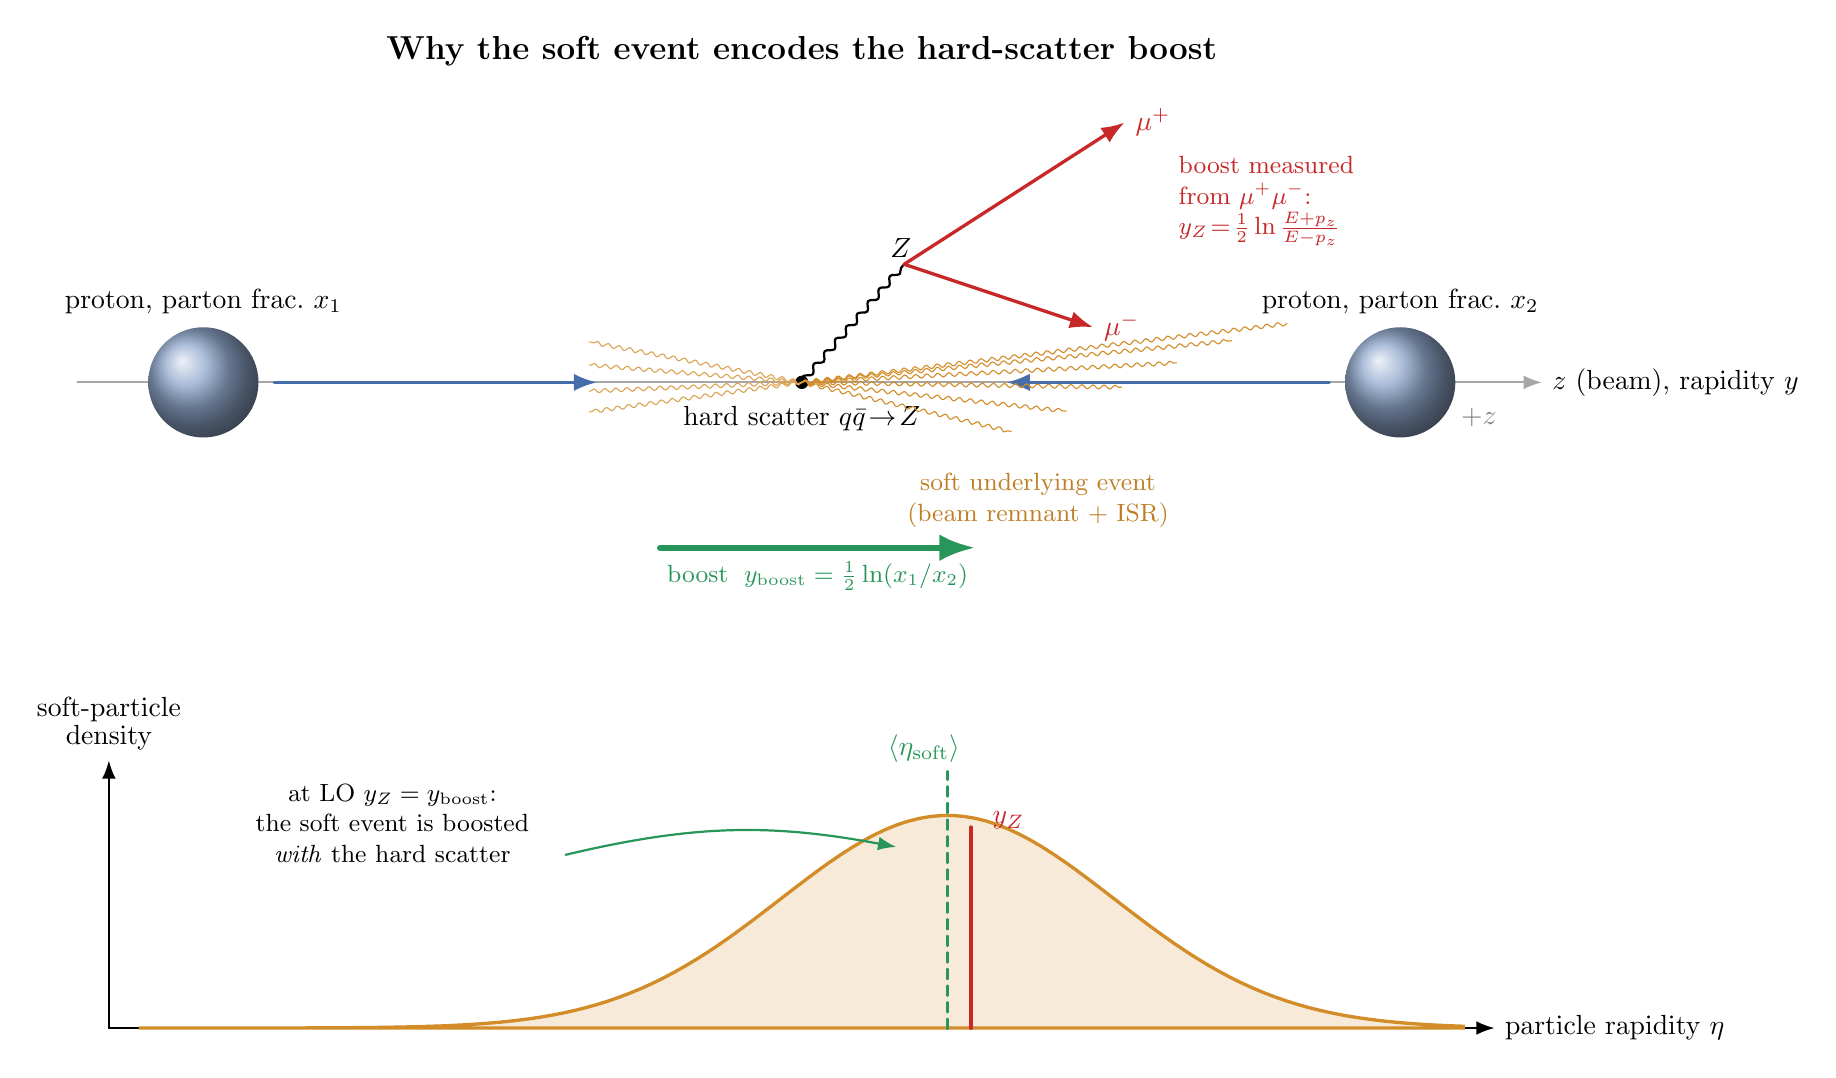
\begin{tikzpicture}[>=Latex,line cap=round]
% ---------- beam axis ----------
\draw[->,thick,gray!70] (-9.2,0) -- (9.4,0) node[right,black]{$z$ (beam), rapidity $y$};
\node[gray] at (8.6,-0.45){$+z$};
% ---------- incoming protons ----------
\shade[ball color=cproton!60] (-7.6,0) circle (0.7);
\shade[ball color=cproton!60] (7.6,0) circle (0.7);
\node[above] at (-7.6,0.75){proton, parton frac.\ $x_1$};
\node[above] at (7.6,0.75){proton, parton frac.\ $x_2$};
\draw[->,very thick,cproton] (-6.7,0) -- (-2.6,0);
\draw[->,very thick,cproton] (6.7,0) -- (2.6,0);
% ---------- hard vertex ----------
\fill[black] (0,0) circle (2.4pt);
\node[below=1pt] at (0,-0.15){hard scatter $q\bar q\!\to\! Z$};
% ---------- Z -> mu mu ----------
\draw[decorate,decoration={snake,amplitude=1.1pt,segment length=6pt},thick] (0,0) -- (1.3,1.5);
\node[right] at (1.0,1.7){$Z$};
\draw[->,very thick,cmuon] (1.3,1.5) -- (4.1,3.3) node[right]{$\mu^+$};
\draw[->,very thick,cmuon] (1.3,1.5) -- (3.7,0.7) node[right]{$\mu^-$};
\node[cmuon,align=left] at (5.9,2.3){\small boost measured\\[-1pt]\small from $\mu^+\mu^-$:\\[-1pt]\small $y_Z\!=\!\tfrac12\ln\frac{E+p_z}{E-p_z}$};
% ---------- beam remnant / soft spray (boosted toward +z) ----------
\foreach \a in {-22,-12,-2,8,18,28}{
  \draw[csoft,decorate,decoration={snake,amplitude=0.7pt,segment length=4pt}]
       (0,0) -- (\a*0.07+4.2, {0.9*sin(\a*2)});}
\foreach \a in {-14,-4,8,20}{
  \draw[csoft!80,decorate,decoration={snake,amplitude=0.7pt,segment length=4pt}]
       (0,0) -- (-2.7, {0.8*sin(\a*2)});}
\node[csoft!90!black,align=center] at (3.0,-1.5){\small soft underlying event\\[-1pt]\small (beam remnant $+$ ISR)};
% ---------- boost arrow (top panel) ----------
\draw[->,line width=2.2pt,cboost] (-1.8,-2.1) -- (2.2,-2.1);
\node[cboost,below] at (0.2,-2.15){\small boost $\;y_{\rm boost}=\tfrac12\ln(x_1/x_2)$};
% ================= lower panel: rapidity distribution =================
\begin{scope}[yshift=-8.2cm]
  \draw[->,thick] (-8.8,0) -- (8.8,0) node[right]{particle rapidity $\eta$};
  \draw[->,thick] (-8.8,0) -- (-8.8,3.4) node[above,align=center]{soft-particle\\[-2pt]density};
  % shifted hill (boosted to +z)
  \def\mu{1.85}
  \draw[csoft,very thick,fill=csoft!18]
     plot[domain=-8.4:8.4,samples=120] (\x,{2.7*exp(-(\x-\mu)*(\x-\mu)/9.0)}) -- (8.4,0) -- (-8.4,0) -- cycle;
  % mean marker
  \draw[cboost,line width=1.4pt,dashed] (\mu,0) -- (\mu,3.25);
  \node[cboost,above] at (\mu-0.3,3.25){$\langle\eta_{\rm soft}\rangle$};
  % y_Z marker
  \draw[cmuon,line width=1.4pt] (2.15,0) -- (2.15,2.55);
  \node[cmuon,above right] at (2.3,2.4){$y_Z$};
  \node[align=center] at (-5.2,2.6){\small at LO $y_Z=y_{\rm boost}$:\\[-1pt]\small the soft event is boosted\\[-1pt]\small \emph{with} the hard scatter};
  \draw[->,cboost,thick] (-3.0,2.2) to[bend left=12] (1.2,2.3);
\end{scope}
% title
\node[font=\bfseries\large] at (0,4.2){Why the soft event encodes the hard-scatter boost};
\end{tikzpicture}
\end{document}
